% \documentclass[../../diplom_data_assimilation.tex]{subfiles}
%use the following makro for all include paths (graphics, data files, other tex files,...)
% \makeatletter\@ifundefined{fromRoot}{\newcommand{\fromRoot}[1]{../../#1}}{}\makeatother
% \begin{document}
\chapter{Datenassimilierung mittels stückweiser Linearisierung}
In diesem Abschnitt widmen wir uns der Aufgabe, das inhomogene adjungierte tangent linear model \eqref{eq:inhAdjEquation} zur verallgemeinerten impliziten Mittelpunktsregel herzuleiten.

\section{Adjoint Inclusion}
\label{sec:adjointInclusion}
Angenommen die rechte Seite $F$ unserer Evolutionsgleichung \eqref{eq:odemodel} sei eine verkettet stückweise glatte Funktion. Dann behält die inhomogene adjungierte Gleichung \eqref{eq:inhAdjEquation} für die glatten Bereiche von $F$ ihre Gültigkeit. An den Nullstellen der switching Variablen $z$ erhalten wir jedoch
\begin{equation}
 \label{eq:adjInclusion}
 \frac{d \delta' x}{dt} =- \partial F(x)^*\delta'x + \nabla H(t)
\end{equation}
Damit ist der Gradient eine mengenwertige Abbildung $\partial F(x)^*:\R^n\rightrightarrows \R^n$ und folglich eine \textit{Differential Inclusion}.
Dadurch ist es möglich, dass in der Zeitintegration Sprünge durch den verallgemeinerten Gradienten $\partial F(x)^*$ auftreten. Falls die Zeitintegration konvergiert, ist deswegen mit einer geringen Konvergenzordnung von ungefähr $\mathcal O(h)$ zu rechnen.
% TODO: Konvergenzresultat?

In der numerischen Berechnung muss der verallgemeinerte Gradient in eine Richtung $\Delta x$ betrachtet werden, sinnvollerweise in die Richtung des Inkrements der vorherigen Iteration $\Delta x_i = x_{i-1} - x_i$, falls wir uns in Iteration $i$ befinden, damit aus der Mengenwertigen Abbildung $ \partial F(x)^*$ ein Gradient ausgewählt wird. 
Falls sich die Gerade $x_i + \Delta x$ auf einem Kink befindet, wie in Abiildung \ref{fig:adjValleyTracing} zu sehen, sprechen wir von einem so genannten \textit{valley tracing mode}, welcher von Khan und Barton in \cite{khan2014} ausführlich behandelt wird. 
\begin{figure}
\centering
\begin{minipage}[b]{0.49\linewidth}
\centering
\documentclass{standalone}
\usepackage{pgfplots,pgfplotstable}

\usetikzlibrary{external}

\begin{document}

\tikzsetnextfilename{adj_valley_tracing}
\begin{tikzpicture}[scale=2]
% Polyhedron
\draw (-0.5,0) -- (0,0.7) -- (1,1) -- (2,0) -- (1,-0.5);
\draw (1,1) -- (1.5,1.5);
\draw (0,0.7) -- (-0.5,1.5);
% Arrow
\draw[->] (1.5,0.5)--(1,0.3);

\draw (1.5,0.5) node {.};
\draw (0.5,0.1) node {.};

\draw (1.5,0.5) node[anchor=west] {$x_i$};

\draw (0.5,0.1) node[anchor=north east] {$x_{i-1}$};
\draw (1.3,0.4) node[anchor=north] {$\Delta x$};
\end{tikzpicture}

 
\end{document}

\caption*{(a) Kink}
\end{minipage}
\begin{minipage}[b]{0.49\linewidth}
\centering
\documentclass{standalone}
\usepackage{pgfplots,pgfplotstable}

\usetikzlibrary{external}

\begin{document}

\tikzsetnextfilename{adj_valley_tracing1}
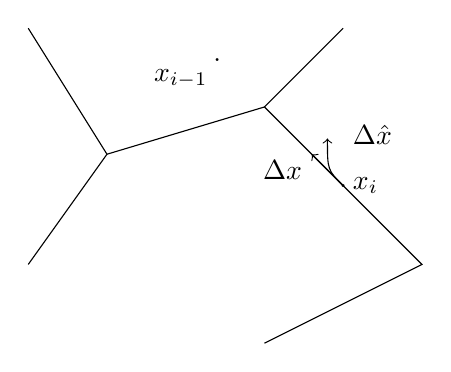
\begin{tikzpicture}[scale=2]
% Polyhedron
\draw (-0.5,0) -- (0,0.7) -- (1,1) -- (2,0) -- (1,-0.5);
\draw (1,1) -- (1.5,1.5);
\draw (0,0.7) -- (-0.5,1.5);
% Arrow
\draw[->] (1.5,0.5)--(1.3,0.7);
\draw (1.3,0.6) node[anchor=east] {$\Delta x$};

% A .. controls B and C .. D
% \draw[->] (1.5,0.5) .. c[swapaxes] (1.2,0.6);
\draw[->] (1.5,0.5) .. controls (1.4,0.6) and (1.4,0.6) .. (1.4,0.8);
\draw (1.5,0.7) node[anchor=south west] {$\Delta \hat x$};

\draw (1.5,0.5) node {.};
\draw (1.5,0.5) node[anchor=west] {$x_i$};

\draw (0.7,1.3) node {.};
 \draw (0.7,1.3) node[anchor=north east] {$x_{i-1}$};

 

\end{tikzpicture}

 
\end{document}

\caption*{(b) Valley tracing mode}
\end{minipage}
\caption{Berechnung der Ableitungsrichtung $\Delta x$ und polynomial escape $\Delta \hat x$ }
\label{fig:adjValleyTracing}
\end{figure}

Eine mögliche Umgehung des Problem des valley tracing modes stellt die Methode des \textit{Polynomial Escapes} dar.
\section{Polynomial Escape}
%agenda:
%brauche Richtung 
%Nehme Richtung zum nächsten Punkt x_i-1 - x_i
%-> Valley tracing mode 
%-> Polynomial escape
%-> Probleme zwischen zwei Stellen mehrere Kinks -> Berechnung am Mittelpunkt 


%TODO Baby example



% \section{Verallgemeinerter Gradient}

% Da die Jacobimatrix an Kinks nicht eindeutig sein muss, wird ein Vektor $d$ mit angegeben, welcher uns die Richtung der Ableitung vorgibt. Diese ist dann wiederum eindeutig bestimmt.
% Um dies mit unseren eben geführten Betrachtungen zu vereinen berechnen wir also den Gradienten $J_\sigma$ nicht an der gegebenen Stelle $x_0$, sondern gehen ein Stück in das durch $d$ und $\Sigma$ vorgegebene Polyeder und berechnen dort die Ableitung an Stelle $\xo_0 = x_0+\frac{1}{2}\tau\cdot d$. Aufgrund der Linearität der Polyeder stimmen die Ableitung an der Stelle $x_0$ und jene an Stelle $\xo_0$ überein. Der Algorithmus ergibt sich sofort zu
% [TODOBild auf Linker Seite]

%TODO BILD POLYNOMIAL ESCAPE
Obwohl es in der Praxis unwahrscheinlich ist, kann der Fall des valley tracing modes eintreten.
%Bei pl data assimilation  brauchen wir polynomial escape
In diesem Fall haben wir keine Bouligandableitung mehr, da das errechnete $\Sigma(z)$ und damit $J_\sigma$ für ein $z_i=0$ Nulleinträge aufweist. Griewank schlägt deshalb in \cite[S.29]{monster} vor, die reduzierte Repräsentation des computational graphs 
\begin{equation}
 \begin{aligned}
  \Delta v_{i-n} &= \Delta x_i \quad \text{für } i=1,\ldots,n, \\
  \Delta z_i &= \sum_{j\prec i} \mathring c_{ij}\Delta v_j,\\
  \sigma_i& = \sign(\mathring z_i + \Delta z_i) \quad \text{für } i=1,\ldots,s,\\
  \Delta v_i &= \sigma_i \cdot (\mathring z_i+\Delta z_i) - \vo_i\\
  \Delta y_{i-s}& = \sum_{j\prec i} \mathring c_{ij} \Delta v_j \quad \text{für } i=s+1, \ldots, s+m
 \end{aligned}
 \label{eq:minComputationalGraphRepr}
\end{equation}
zu nutzen, wobei $\mathring c_{ij}$ die glatten Ableitungen zum Entwicklungspunkt $\xo$ bezeichnen und mit Hilfe Dieser den sogenannten \textit{polynomial escape} anzuwenden. In Abs Normal Form ist die obere Prozedur äquivalent dazu, die Ableitung der Abs-Normal Form 
\begin{equation}
\begin{aligned}
  \Delta z = Z\Delta x + L\Sigma \Delta z \\
 \Delta y = J\Delta x + Y\Sigma \Delta z  
\end{aligned}
\label{eq:jacAbsNormalForm}
\end{equation}
für $\Sigma = \diag(\sigma) \in \R^{s\times s}$ zu berechnen. Die Idee besteht nun darin, die Richtung $\Delta x$, in der der Gradient berechnet werden soll, in den Nulleinträgen so zu stören, dass wir uns innerhalb eines Polyeders befinden, der Rest jedoch unangetastet bleibt. Da das Komplement $\mathcal C$ aller offenen Polyeder $P_\sigma$ aus eine endliche Anzahl an Hyperflächen  besteht kann kein Pfad der Form
\begin{equation}
 \Delta x(t) = \sum_{j=1}^n e_j t^j \quad ,0<t<\bar t;~e_j\in \R^n ~,\det(e_1,\ldots,e_n)\neq 0
\end{equation}
für eine Schranke $\bar t$ auf diesen Hyperflächen liegen (\cite[Proposition 6]{monster},\cite[S.11]{plan}). 
Ein naheliegender Ansatz ist die Auswertungsprozedur \eqref{eq:jacAbsNormalForm} mit den Signaturen
\[
 \sigma_i = \text{firstsign}(z_i,\nabla z_i^\tr\Delta x) = \sign(z_i+\Delta z_i)
\]
anzuwenden. Hierbei ist firstsign$(z,\Delta z)$ eines Vektors $z$ definiert ist als das Vorzeichen der ersten nicht verschwindenden Komponente des Vektors $z$, ansonsten wird sie zu $\Delta z$ gesetzt. Falls nun alle Werte $\sigma_i \neq 0$ sind, ist $J_\sigma$ eine Bouligandableitung der Funktion $F$ und ihrer stückweisen Linearisierung im Polyeder $P_\sigma$ auf dessen Abschluss der Auswertungspunkt $\xo$ liegt (\cite[S.]{monster}).

Der Ansatz um diesen Pfad zu konstruieren besteht darin, den Richtungsvektor $e_1 = \Delta x$ mit $n-1$ linear unabhängigen Vektoren $e_2,\ldots, e_n$ zu komplementieren, sodass sie eine nichtsinguläre Basismatrix $E\in \R^{n\times n}$ bilden.
Das bedeutet, wir stellen das System linear unabhängiger Vektoren $\tilde E$, welche wir definieren als
\[
\tilde E = 
 \begin{pmatrix}
  \vdots   & I_{n-k} & 0 \\
  \Delta x_k & 0&0\\
  \vdots   & 0&I_{k-1}
 \end{pmatrix}
\]
Dabei ist $\Delta x_k$ der Eintrag mit dem betragsmäßig größten, nicht verschwindenden Element und $I$ die Einheitsmatrix. Nun verschieben wir durch eine Permutationsmatrix $P$ den Vektor $\Delta x$ an die $k$-te Stelle der Matrix $\tilde E$
\[
E = \tilde E \cdot P=
\begin{pmatrix}
  \nabla x_1^\tr\\
  \vdots\\
  \nabla x_n^\tr\\
 \end{pmatrix}
 =
  \begin{pmatrix}
   I_{n-k} & \vdots &0\\
  0 & \Delta x_k & 0\\
    0 & \vdots&I_{k-1}
 \end{pmatrix}
\]
Diese Permutation ist numerisch von großer von Bedeutung. $E$ kann geschrieben werden als
\[
  E = I + (\Delta x-e_k)\cdot e_k^\tr 
\] 
deren Inverse sich nach der \textit{Sherman-Morrison-Woodbury} Formel zu folgendem Ausdruck ergibt 
\[
 E^{-1} = I + \frac{(\Delta x-e_k)\cdot e_k^\tr}{\Delta x_k}
\]
Da $\tilde E$ zu $E$ permutiert wurde, ist sichergestellt, dass das Inverse $E^{-1}$ die bestmögliche numerische Genauigkeit der Division behält.
Die $\sigma_i$ erhalten wir nun lexikographisch, indem wir Prozedur \eqref{eq:jacAbsNormalForm} auf jeden Vektor aus $E$ anwenden mit 
\[
  \sigma_i = \text{firstsign}(z_i,\nabla z_i^\tr\Delta x)
\]

Griewank konnte in \cite[Prop.8]{monster} zeigen, dass solch eine permutierte lexikographische Definition von $\sigma_i$ ebenfalls zu einer limiting Jacobian führt
% Falls nun die Jacobimatrix auf einem Kink berechnet werden soll, ist sie nicht mehr eindeutig. 
\begin{theorem}[Polynomial Escape]
Angenommen, wir initialisieren $(\nabla x_i^\tr)_{i=1,\ldots,n} = E$ mit $\det(E)\neq 0$ und sei $\sigma$ lexikographisch bestimmt. Dann ergibt die Auswertung von Gleichung \eqref{eq:jacAbsNormalForm} eine Matrix $J_\sigma^E = (\nabla y_{i-s}^\tr)_{i=1,\ldots,m}$ dessen Rücktransformation
\[
 J_\sigma \equiv J_\sigma^E E^{-1} \in \partial^L \Delta F(\xo;0) 
\]
eine limiting Jacobian von $F'(\xo;\Delta x))$ und $\Delta F(\xo;\Delta x)$ am Punkt $\xo$ ist.
\end{theorem}
Der Algorithmus \ref{alg:polynomialEscape} zeigt die zur Berechnung benötigten Schritte.
 \begin{algorithm}
 \algrenewcommand{\algorithmiccomment}[1]{\hfill{\scriptsize #1}}
 \caption{Polynomial Escape}
 \label{alg:polynomialEscape}
 \begin{algorithmic}[1]
 \Function{gen\_jac}{$x,\Delta x$}
 	\State $k \gets \max_i\lbrace i~|~\Delta x_i\rbrace$
 	\State $z \gets $calculate\_z($x$)
 	\For{$i=1\ldots n$}\Comment{Berechnung von $\nabla z$}
	  \State $\sigma_i\gets \sign(z_i)$ 
	  \State $\nabla z_{i,1} = Z.row(i)\cdot \Delta x$\Comment{Berechne $Z\Delta x$}
	  \State $\nabla z_{i,j+1} = Z.row(i)\cdot e_j$, für $j=1,\ldots,k-1$
	  \State $\nabla z_{i,j} = Z.row(i)\cdot e_j$, für $j=k+1,\ldots, n$
	  \State $\nabla z.row(i) \mathrel{+}= L_{i,j}\cdot \sigma_j\cdot \nabla z.row(j)$ für $j=1,\ldots, i$\Comment{Berechne $L\Sigma \nabla z$}
	  \State $j\gets 2$
	  \While{$\sigma_i==0$ \&\& $j<s$ }\Comment{Firstsign}
	    \State $\sigma_i \gets \sign(\nabla z_{i,j})$
	    \State $j++$
	  \EndWhile
	\EndFor
	\For{$i=1\ldots n$}\Comment{Berechnung von $\nabla y$}
	  \State $\nabla y_{i,1} = J.row(i)\cdot \Delta x$\Comment{Berechne $J\Delta x$}
	  \State $\nabla y_{i,j+1} = J.row(i)\cdot e_j$, für $j=1,\ldots,k-1$
	  \State $\nabla y_{i,j} = J.row(i)\cdot e_j$, für $j=k+1,\ldots, n$
	  \State $\nabla y.row(i) \mathrel{+}= Y_{i,j}\cdot \sigma_j\cdot \nabla z.row(j)$ für $j=1,\ldots, n$\Comment{Berechne $Y\nabla z$}
	\EndFor
	\For{$j=1\ldots n$}\Comment{Berechnung von $J_\sigma^E\cdot E^{-1}$}
	  \State $\tilde J_{i,j} =\nabla y_{j,i+1}$für $i=1,\ldots,k-1$
	  \State $\tilde J_{i,j} = \nabla y_{j,i} $ für $i=k+1,\ldots,n$
	  \State $\tilde J_{k,j} = \nabla y_{j,1}$
	  \State $\tilde J_{k,j} \mathrel{+}= (\tilde J_{i,j}\Delta x_i) / \Delta x_k$ für $i=1,\ldots,k-1,k+1,\ldots,n$
	\EndFor
	\State $J_\sigma = \tilde J$
 \EndFunction
 \end{algorithmic}
 \end{algorithm}
% Für die Inhomogene Adjungierte Gleichung ergibt sich
% \[
%  \frac{d \delta' x}{dt} =- F'(x;\Delta x)^\tr\delta'x + \nabla H(t)
% \]
% Der
% Ein auf diese Weise berechneter verallgemeinerter Gradient 
% TODO: Dieser verallgemeinerte Gradient ist wenigstens im Abschluss von $P_\sigma$ ein gradient oder so (nachschauen wo der Satz kam) 
% TODO: Bezug nehmen auf aktuelle Forschung von Andreas (short und so) -> reicht im Ausblick?
%% GENERALIZED ADJOINT MIDPOINT RULE
\section{Adjungierte verallgemeinerte Mittelpunktsregel}

% Wie wir in (??) beobachtet haben, müssen wir das Adjungierte Modell rückwärts integrieren. Die Grundidee besteht darin, dass wir auf das Adjungierte Modell (??) der Datenassimilierung ebenfalls wieder die verallgemeinerte Mittelpunktsregel (??) anwenden. Daher, dass wir das Integral in Teilintervalle zerlegen können, berechnen wir die kritischen Multiplikatoren, springen von Kink zu Kink und berechnen auf diesen Teilintervalen den Gradienten unserer rechten Seite $F$.
In diesem Abschnitt wollen wir die inhomogene adjungierte Differentialgleichung auf die verallgemeinerte Mittelpunktsregel anwenden.

Falls wir den Gradienten des Kostenfunktionals mit der impliziten Mittelpunktsregel berechnen, so würden wir als Auswertungspunkt des Gradienten den Mittelpunkt $\xo$ benutzen. Wie in Abbildung \ref{fig:multipleKinksAdjoint}(a) zu erkennen ist, kann dies dazu führen, dass der Gradient keine sinnvolle Aussage der Steigung widerspiegelt. Im Rolling Stones Beispiel (\ref{sec:rollingStonesExample}) mündet dieses Problem beispielsweise in einem sehr verzerrten Gradienten (siehe Abbildung \ref{fig:rollingGrad}). Wir wollen nun die Eigenschaften der verallgemeinerten impliziten Mittelpunktsregel nutzen, um eine Art Mittelwert des Gradienten berechnen zu können, der an den Stellen zwischen den Kinks, wie in Abbildung \ref{fig:multipleKinksAdjoint}(b), ausgewertet und gewichtet summiert wird. 

\begin{figure}
\footnotesize
\centering
\begin{minipage}[b]{\linewidth}
% \begin{minipage}[t][3cm][t]{5cm}
\documentclass{standalone}
\IfStandalone{
	\usepackage{pgfplots,pgfplotstable}
	\usetikzlibrary{external}
	\newcommand{\fromRoot}[1]{../#1}
}{%
}\begin{document}

\tikzsetnextfilename{multiple_kinks_adjoint}
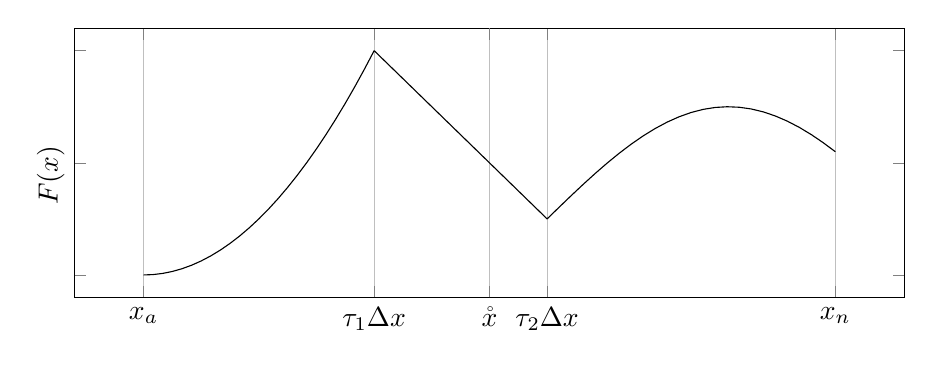
\begin{tikzpicture}
\begin{axis}[
	width=\linewidth,
	height=5cm,
	xmajorgrids,
	xtick={0,2,3.5,6},
	xticklabels={$ x_a$,$\tau_1\Delta x$,$\tau_2\Delta x$,$x_n$},
	yticklabel=\empty,
	ylabel={$F(x)$},
	every axis y label/.style={
	  rotate=90,
	  at={(ticklabel* cs:0.6)},
	  anchor=south east,
	},
	extra x ticks={3},
	extra x tick labels={$\mathring x$}
]
	\addplot [mark=none,draw=black,thin, domain=0:2] {0.5*x^2};
	\addplot [mark=none,draw=black,thin, domain=2:3.5] {-x+4)};
	\addplot [mark=none,draw=black,thin, domain=3.5:6] {sin(deg(x-3.5))+0.5};
\end{axis}

\end{tikzpicture}

 
\end{document}

\caption*{(a) Klassische implizite Mittelpunktsregel}
\end{minipage}
\begin{minipage}[b]{\linewidth}
% \begin{minipage}[t][3cm][t]{5cm}
\documentclass{standalone}
\usepackage{pgfplots,pgfplotstable}

\usetikzlibrary{external}

\begin{document}

\tikzsetnextfilename{multiple_kinks_adjoint_new}
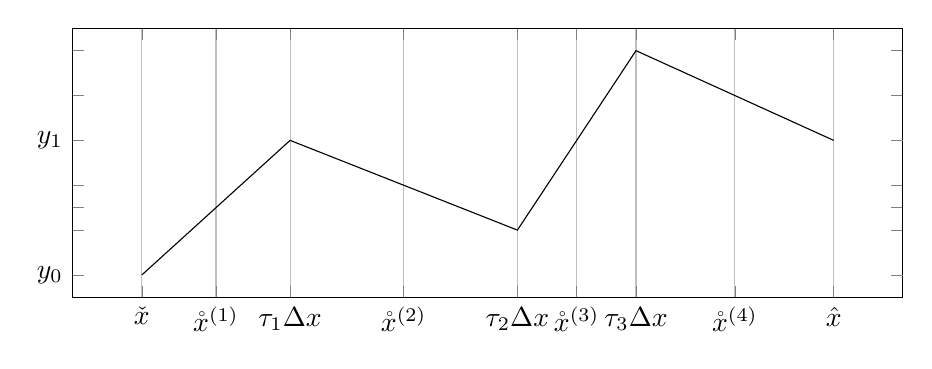
\begin{tikzpicture}
% \draw (0,0) grid (7,3);
% \draw[help lines,->] (0,0) -- (7,0) node[anchor=north west] {$v$};
% \draw[help lines,->] (0,0) -- (0,3) node[anchor=south east] {$y$};
% 
% \draw (0,1) -- (1,2) -- (2,0.5) -- (3,1.5) -- (4,1) -- (5,2.5) -- (6,2);
\begin{axis}[
	width=\linewidth,
	height=5cm,
% 	xlabel = $v$,
% 	ylabel = $y$,
	xtick = data,
	ytick = data,
	xmajorgrids,
	xticklabels={ $\check x$,
		      $\mathring x^{(1)}$,
		      $\tau_1\Delta x$,
		      $\mathring x^{(2)}$,
		      $\tau_2 \Delta x$,
		      $\mathring x^{(3)}$,
		      $\tau_3 \Delta x$,
		      $\mathring x^{(4)}$,
		      $\hat x$},
	yticklabel=\empty,
	extra y ticks={1,1.3},
	extra y tick labels={$y_0$,$y_1$},
]
	\addplot[no marks] table {
		0 1
		0.75 1.15
		1.5 1.3
		2.65 1.2
		3.8 1.1
		4.4 1.3
		5 1.5
		6 1.4
		7 1.3
	};
% 	fmeow
\end{axis}

\end{tikzpicture}

 
\end{document}

\caption*{(b) Verallgemeinerte implizite Mittelpunktsregel}
\end{minipage}
\caption{Punkte $\xo$ der Gradientberechnung in der Adjungierten Gleichung}
\label{fig:multipleKinksAdjoint}
\end{figure}


Sei dazu $\tau$ der kritische Multiplikator zum nächsten Kink. $x_n$ und $x_a$ sind die jeweiligen iterierten Werte mit $\xo$ als deren Mittelpunkt und $\diff \xo$ als Differenz. Folglich ergibt sich 
\begin{align*}
\xo &= \frac{x_n+x_a}{2}\eq x_a = 2\xo - x_n\\
\diff \xo &= \xo_n - \xo_a \eq \xo_n = \diff \xo + \xo_a\\
x_n - x_a &= 2x_n - 2\xo\\
\diff \tau_j&=\tau_j-\tau_{j-1}
\end{align*}
Die inhomogene adjungierte Differentialgleichung ergibt sich aus \eqref{eq:inhAdjEquation} mit adjungierter Variable $\xadj := \gatdiff x$ zu
\begin{equation}
\dot{\xadj} = x - x_{obs} - \frac{\partial F(x,d)}{\partial x}^\tr \cdot \xadj
\label{eq:adjModel}
\end{equation}

Wenn nun die verallgemeinerte Mittelpunktsregel \eqref{eq:genMidpointRule} auf die Gleichung \eqref{eq:adjModel} angewendet wird, folgt
\begin{align*}
\xadj_n - \xadj_a &= h\cdot \int_{-0.5}^{0.5}\xo-\rxobs - \frac{\partial F(\xo,d)}{\partial x}^\tr \cdot \xadj\\
									&= h\cdot \left[\xo-\rxobs - \int_{-0.5}^{0.5} \frac{\partial F(\xo ,d)}{\partial x}^\tr \cdot \xadj dt\right]\\
\end{align*}
Angenommen es existieren $l \in \mathbb{N}$ Kinks zwischen $x_n$ und $x_{a}$, wobei \[-0.5 = \tau_0 <\tau_1 <\ldots < \tau_l=0.5\] gilt, dann kann durch die Additivität das Integral aufgespalten werden, sodass wir über die Teilintervalle $[t_j,t_j+1], j=0,\ldots,l$ integrieren und unabhängige Variablen herausziehen können:
\begin{align*}
\xadj_n - \xadj_a &= h\cdot \left[ \xo-\rxobs - \sum_{i=1}^l \int_{\tau_{i-1}}^{\tau_{i}}\frac{\partial F(\xo+\tau_{i-1}d,d)}{\partial x}^\tr \cdot \xadj dt\right]\\
									&= h\cdot \left[\xo -\rxobs - \sum_{i=1}^l \underbrace{\frac{\partial F(\xo+\tau_{i-1}d,d)}{\partial x}^\tr }_{A_i^\tr} \cdot \int_{\tau_{i-1}}^{\tau_{i}} \xadj dt\right]\\
\end{align*}

Nun wird die stückweise Linearisierung auf $\xadj$ angewendet. Es entsteht
\allowdisplaybreaks
\begin{align*}
\xadj_n - \xadj_a &= h\cdot (\xo -\rxobs - \sum_{i=1}^l A_i^\tr \cdot \int_{\tau_{i-1}}^{\tau_{i}} \rxadj + t\diff \xadj dt)\\
		  &= h\cdot \left[\xo -\rxobs - \sum_{i=1}^l A_i^\tr \cdot \left[t\rxadj + \frac{t^2}{2}\diff \xadj \right]_{\tau_{i-1}}^{\tau_i} \right]\\
		  &= h\cdot \left[\xo -\rxobs - \sum_{i=1}^l A_i^\tr \cdot \left( (\tau_i - \tau_{i-1})\cdot \rxadj + \frac{1}{2}\diff \xadj \cdot(\tau_i^2-\tau_{i-1}^2) \right)\right]\\
		  &= h\cdot \left[\xo -\rxobs - \sum_{i=1}^l A_i^\tr \cdot \left(\diff \tau_i\cdot \rxadj +  \diff \tau_i \frac{1}{2}\cdot(\tau_i+\tau_{i-1})\cdot \diff \xadj \right)\right]\\
		  &= h\cdot \left[\xo -\rxobs - \sum_{i=1}^l A_i^\tr \cdot \left( \diff \tau_i\cdot \rxadj +  \diff \tau_i \rtau_i \diff \xadj \right)\right]
\end{align*}

Mit $\rxadj =\frac{1}{2}(\xadj_n + \xadj_a) $ und $\diff \xadj =\xadj_n - \xadj_a $ ergibt sich
\allowdisplaybreaks
\begin{align*}
\xadj_n - \xadj_a &= h\cdot \left[\xo -\rxobs - \sum_{i=1}^l A_i^\tr \cdot \left( \diff \tau_i\cdot \frac{\xadj_n + \xadj_a}{2} +  \diff \tau_i \rtau_i (\xadj_n - \xadj_a) \right)\right]\\
 &= h\cdot \left(\xo -\rxobs\right) \\
 &\quad-h\left[\sum_{i=1}^l A_i^\tr \cdot \left( \left(\frac{1}{2} \diff \tau_i +\diff \tau_i \rtau_i\right) \cdot \xadj_n  +  \left(\frac{1}{2}\diff \tau_i-\diff \tau_i \rtau_i\right) \cdot \xadj_a \right)\right]\\
 &= h\cdot \left(\xo -\rxobs \right)\\
 &\quad-h \left[\left( \sum_{i=1}^l A_i^\tr \left(\frac{1}{2} \diff \tau_i +\diff \tau_i \rtau_i\right) \cdot \xadj_n  + \sum_{i=1}^l A_i^\tr  \left(\frac{1}{2}\diff \tau_i-\diff \tau_i \rtau_i\right) \cdot \xadj_a \right)\right]\\
\end{align*}
 
Durch Umsortierung erhalten wir
\begin{equation}
\label{eq:genMidpointAdjoint}
\begin{aligned}
&& \left[I +h\sum_{i=1}^l A_i^\tr \left(\frac{1}{2} \diff \tau_i +\diff \tau_i \rtau_i\right) \right]\xadj_n &= 
\begin{aligned}[t]
&\left[I - h\sum_{i=1}^l A_i^\tr  \left(\frac{1}{2}\diff \tau_i-\diff \tau_i \rtau_i\right)\right]\xadj_a \\
& +h (\xo -\rxobs)
\end{aligned}\\
\iff&& \left[I +\frac{h}{2} \bar{A}^\tr +h\hat{A}^\tr\right]\xadj_n &= \left[I - \frac{h}{2}\bar{A}^\tr + h\hat{A}^\tr\right]\xadj_a  +h (\xo -\rxobs)\\
\end{aligned}
\end{equation}
mit $\bar{A}^\tr = \sum_{i=1}^l A_i^\tr \diff \tau_i $ und $\hat{A}^\tr = \sum_{i=1}^l A_i^\tr \diff \tau_i \rtau_i$.
Als Algorithmus ergibt sich folglich Prozedur 4, welche die Berechnung von $\bar A$ und $\hat A$ durchführt, als auch Prozedur 5, welche das erstellte Gleichungssystem löst.
 \begin{algorithm}[H]
 \algrenewcommand{\algorithmiccomment}[1]{\hfill{\scriptsize #1}}
 \caption{Gewichtete Gradienten}
 \label{alg:kinkPartials}
 \begin{algorithmic}[1]
 \Function{calc\_kink\_partial}{$\cx,\hx,\Delta x$}
 	\State $\hat{\tau} \gets 0$, $x_{kink} \gets \cx$
 	\State $\bar{A} \gets 0 $, $\hat{A} \gets 0$
 	\Repeat
 	  \State $\check{\tau} \gets \check{\tau} + \hat{\tau}, ~ x_{kink} \gets x_{kink} +\check{\tau}\Delta x$
 	  \State $\hat{\tau} \gets \check{\tau} + \Call{critMult}{ x_{kink},\Delta x}$ 		 \Comment{Berechne kritischen Multiplikator}
		\If{$\hat{\tau}>1$} $\hat{\tau}\gets 1$ \EndIf 
 		\State $\rx \gets x_{kink}+0.5\cdot \hat{\tau} \Delta x$	\Comment{Berechne Mittelpunkt zwischen den Kinks}
 	  \State $\frac{\partial F(\rx)}{\partial x} \gets $ gen\_jac($\rx,\Delta x$) \Comment{Berechne $\partial F$ aus der Abs-Normalform}
 
 % 		\State $\rx \gets \Call{Solve}{\rx_\mathrm{new}}$
 	  \State $\bar{A} \gets \bar{A} +  \frac{\partial F(\rx)}{\partial x} \cdot (\hat{\tau} - \check{\tau})$ 
 		\State $\hat{A} \gets \hat{A} +  \frac{\partial F(\rx)}{\partial x} \cdot  \left(\frac{1}{2}(\check{\tau} + \hat{\tau})-0.5\right)$ \Comment{Verschiebe $\tau$ um $-0.5$}
 		
 \Until{$\hat{\tau} \geq 1$	}
 \State \Return $[\bar{A}, \hat{A}]$;
 \EndFunction
 \end{algorithmic}
 \end{algorithm}
\begin{algorithm}
 \algrenewcommand{\algorithmiccomment}[1]{\hfill{\scriptsize #1}}
 \caption{Gradient des Kostenfunktionals}
 \label{alg:jacDataAssimilation}
 \begin{algorithmic}[1]
%  \Require $x_{0},t_0,T, h,x_{Obs}, TOL$
 \Function{jac\_data\_assimilation}{$x_{0},t_0,T, h,x_{Obs}, TOL$}
 \State $N = \ceilS{\frac{t_0 - T}{h}}$
 \State $\hat{\bar{x}} \gets 0$ \Comment{Setze Anfangswert}
 \State $x \gets  \Call{solveODE}{x_0,t_0, T,h, TOL};$\Comment{Löse ODE in Vorwärtsrichtung}
 \For{$k\gets$ N-1 to $1$} \Comment{Zeitschritt rückwärts}
 	%\State $\rx \gets \cx - \frac h2 F(\cx)$ \Comment{initialization by half Euler}
 	\State $\rx \gets 0.5(x_k + x_{k-1})$ \Comment{Berechne Mittelpunkt}
 	\State $\pl_{\rx} F \gets \Call{Update}{}$ \Comment{Berechne neue Linearisierung am Mittelpunkt $\rx$}
 	\State $\Delta x \gets x_{k-1}-x_k$\Comment{Berechne neue Richtung}
 	\State $[\bar{A},\hat{A}] \gets \Call{calc\_kink\_partials}{x_k,x_{k-1},\Delta x}$  \Comment{Berechne $\partial F$ zwischen jedem Kink}
 	%\Until{$\|\hx - \cx - r - h F(\rx)\|$} < TOL
 	\State $\check{\bar{x}} \gets \Call{Solve}{( I-\frac{h}{2}\bar{A}^\tr + h \hat{A}^\tr)\check{\bar{x}}  = (I+\frac{h}{2}\bar{A}^\tr + h\hat{A}^\tr)\hat{\bar{x}}- h(\rx-\rx_{Obs})}$
 \EndFor
 \State \Return $-\check{\bar{x}}$
 \EndFunction
 \end{algorithmic}
 \end{algorithm}
Bemerkt sei, dass sich die Formel für $l=1$, wenn sich also kein Kink zwischen $x_n$ und $x_a$ befindet, zur bekannten impliziten Mittelpunktsregel vereinfacht. Für diesen Fall gilt $\diff \tau =1,\rtau = 0$ und damit
\begin{align*}
&& \left[I +h\sum_{i=1}^1 A_i^\tr \left(\frac{1}{2} \diff \tau_i +\diff \tau_i \rtau_i\right) \right]\xadj_n &=\begin{aligned}[t]
   & \left[I - h\sum_{i=1}^1 A_i^\tr  \left(\frac{1}{2}\diff \tau_i-\diff \tau_i \rtau_i\right)\right]\xadj_a  \\
	&+	h\cdot (\xo -\rxobs) 
       \end{aligned} \\
\iff &&  \left[I +h A_1^\tr \left(\frac{1}{2} \diff \tau_1 +\diff \tau_1 \rtau_1\right) \right]\xadj_n &= 
  \begin{aligned}[t]	
&\left[I - h A_1^\tr  \left(\frac{1}{2}\diff \tau_1-\diff \tau_1 \rtau_1\right)\right]\xadj_a  \\
&+h\cdot (\xo -\rxobs)
  \end{aligned} \\
\iff &&  \left[I +h A_1^\tr \left(\frac{1}{2} \cdot 1+0\right) \right]\xadj_n &= \begin{aligned}[t]
&\left[I - h A_1^\tr  \left(\frac{1}{2} \cdot 1-0\right)\right]\xadj_a \\
&+h\cdot (\xo -\rxobs)                                                                                  
\end{aligned}\\
\iff &&  \left[ I +\frac{h}{2} \frac{\partial F(\xo ,d)}{\partial x}^\tr \right]\xadj_n &= 
\begin{aligned}[t]
&\left[ I - \frac{h}{2}  \frac{\partial F(\xo ,d)}{\partial x}^\tr  \right]\xadj_a \\
&+h\cdot (\xo -\rxobs)\\
\end{aligned}\\
\iff &&  \xadj_n - \xadj_a &=h\cdot \left[\xo -\rxobs - \frac{\partial F(\xo ,d)}{\partial x}^\tr  \frac{\xadj_n + \xadj_a}{2}\right]\\
\end{align*}
Dies entspricht der verallgemeinerten impliziten Mittelpunktsregel \eqref{eq:genMidpointRule} für das inhomogene adjungierte Modell \eqref{eq:adjModel}.
 

 
\section{Optimierung}
 Zur Zeit der Erstellung dieser Arbeit konnte keine sinnvolle Verbesserung der Optimierung des Kostenfunktionals gefunden werden. Es wird daher das BFGS Verfahren benutzt, welches nach Zou und Navon in \cite{zou1993numerical} gute Ergebnisse für die 4-D Datenassimilierung liefert. 